%%%%%%%%%%%%%%%%%%%%%%%%%%%%%%%%%%%%%%%%%
% Beamer Presentation
% LaTeX Template
% Version 1.0 (10/11/12)
%
% This template has been downloaded from:
% http://www.LaTeXTemplates.com
%
% License:
% CC BY-NC-SA 3.0 (http://creativecommons.org/licenses/by-nc-sa/3.0/)
%
%%%%%%%%%%%%%%%%%%%%%%%%%%%%%%%%%%%%%%%%%

%----------------------------------------------------------------------------------------
%	PACKAGES AND THEMES
%----------------------------------------------------------------------------------------

\documentclass{beamer}

\mode<presentation> {

% The Beamer class comes with a number of default slide themes
% which change the colors and layouts of slides. Below this is a list
% of all the themes, uncomment each in turn to see what they look like.

%\usetheme{default}
%\usetheme{AnnArbor}
%\usetheme{Antibes}
%\usetheme{Bergen}
%\usetheme{Berkeley}
%\usetheme{Berlin}
%\usetheme{Boadilla}
%\usetheme{CambridgeUS}
%\usetheme{Copenhagen}
%\usetheme{Darmstadt}
%\usetheme{Dresden}
%\usetheme{Frankfurt}
%\usetheme{Goettingen}
%\usetheme{Hannover}
%\usetheme{Ilmenau}
%\usetheme{JuanLesPins}
%\usetheme{Luebeck}
%\usetheme{Madrid}
%\usetheme{Malmoe}
%\usetheme{Marburg}
%\usetheme{Montpellier}
%\usetheme{PaloAlto}
\usetheme{Pittsburgh}
% \usetheme{Rochester} % molto pulito
%\usetheme{Singapore} % Molto bello, l'unica cosa e' levare i sottotitoli
%\usetheme{Szeged}
%\usetheme{Warsaw}

% As well as themes, the Beamer class has a number of color themes
% for any slide theme. Uncomment each of these in turn to see how it
% changes the colors of your current slide theme.

%\usecolortheme{albatross}
%\usecolortheme{beaver}
%\usecolortheme{beetle}
%\usecolortheme{crane}
%\usecolortheme{dolphin}
%\usecolortheme{dove}
%\usecolortheme{fly}
%\usecolortheme{lily}
%\usecolortheme{orchid}
%\usecolortheme{rose}
%\usecolortheme{seagull}
%\usecolortheme{seahorse}
%\usecolortheme{whale}
%\usecolortheme{wolverine}

%\setbeamertemplate{footline} % To remove the footer line in all slides uncomment this line
%\setbeamertemplate{footline}[page number] % To replace the footer line in all slides with a simple slide count uncomment this line

%\setbeamertemplate{navigation symbols}{} % To remove the navigation symbols from the bottom of all slides uncomment this line
}

\usepackage{graphicx} % Allows including images
\usepackage{booktabs} % Allows the use of \toprule, \midrule and \bottomrule in tables
\usepackage{textpos}
\usepackage{hyperref}
\usepackage{movie15}
%----------------------------------------------------------------------------------------
%	TITLE PAGE 1
%----------------------------------------------------------------------------------------
\begin{document}

 \title[BTech Project]{\vspace{0.15cm}Embedded Systems Project Presentation:\\TEG Characterization}  % The short title appears at the bottom of every slide, the full title is only on the title page
  \author[Giacomo Mazzucchi and Filippo Faccini]{ Giacomo Mazzucchi and Filippo Faccini
\scriptsize
 }
\institute[UniTn]{

\includegraphics[scale=0.1]{images/logo_unitn.jpg}
\newline
\\\footnotesize{Dept. of Industrial Engineering\\University of Trento} % Your institution for the title page
}
%\date{March xx, 2023}
\scriptsize{\date{\today}} % Date, can be changed to a custom date



%\begin{frame}
%\titlepage % Print the title page as the first slide
%\end{frame}


%----------------------------------------------------------------------------------------
%	TITLE PAGE
%----------------------------------------------------------------------------------------

\begin{frame}
\titlepage 
\end{frame}


\begin{frame}
\frametitle{Overview} 
\tableofcontents 
\end{frame}

%----------------------------------------------------------------------------------------
%	PRESENTATION SLIDES
%----------------------------------------------------------------------------------------

%------------------------------------------------
\section{Introduction}

\begin{frame}
	\frametitle{Problem Goal}

\subsection{Project Goal}
\begin{block}{TEG Characterization}
\begin{itemize}
    \item Thermoelectric generators are devices that convert heat into electrical energy
    \item Their behaviour is regulated by a model based on three key parameters: \textbf{Seebeck coefficient}, \textbf{electrical resistance} and \textbf{thermal conductivity}
    %\begin{enumerate}
    %    \item Seebeck coefficient
    %    \item Electrical resistance
    %    \item Thermal conductivity
    %\end{enumerate}
\end{itemize}
\end{block}

    \begin{figure}
        \centering
        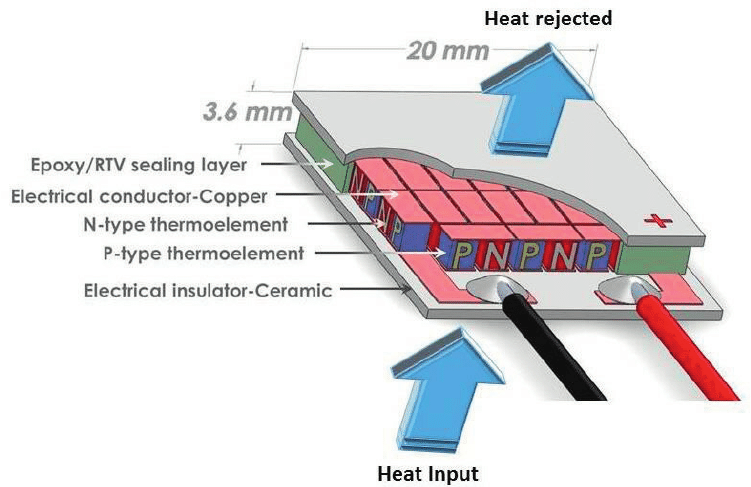
\includegraphics[scale=0.20]{images/TEG_Example.png}
        \caption{Thermoelectric Generator}
    \end{figure}
\end{frame}

\begin{frame}
    \frametitle{Steps}

\subsection{Steps}
\begin{block}{Steps to find the model of a specific TEG device}
\begin{enumerate}
    \item Generate a known delta temperature between two sides of TEG
    \item Measure Open Circuit voltage
    \item Estimate Seebeck coefficient
    \item Measure current on a known load resistor
    \item Estimate internal resistance
    \item Calculate efficiency of the TEG	
\end{enumerate}
\end{block}
\end{frame}

%------------------------------------------------

% \subsection{Subsection Example} % A subsection can be created just before a set of slides with a common theme to further break down your presentation into chunks
\section{Data collection}
\subsection{HW Setup}
\begin{frame}
    \frametitle{HW Setup}
    
\begin{block}{Components}
    \begin{itemize}
        \item A \textbf{wire wound resistor}, used as hot side heating element
        \item Hot side control circuit, composed of a transistor and a \textbf{power MOSFET}
        \item Temperature acquisition, with the \textbf{MAX6675 module}
        \item Open circuit voltage measurement with the ADC of the MCU
        \item Current measurements using the MicroCurrent module
    \end{itemize}
\end{block}

\begin{figure}
        \centering
        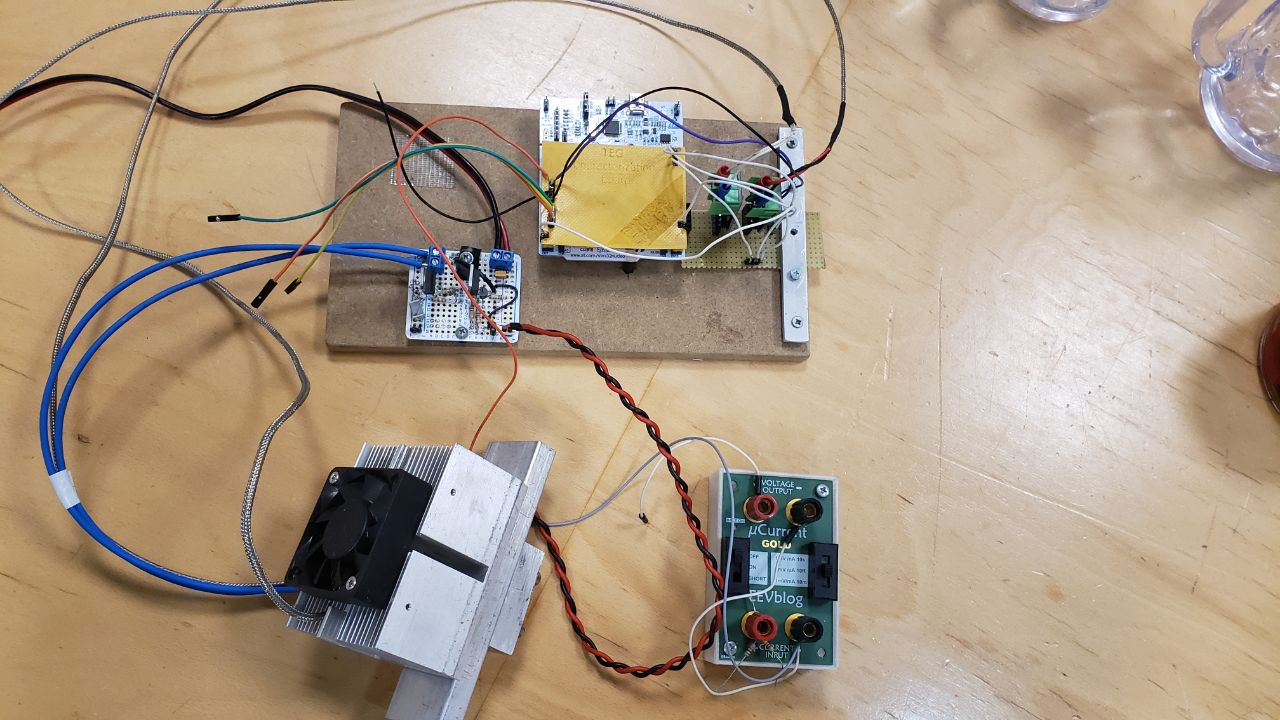
\includegraphics[scale=0.15]{images/tegsetup.jpg}
        \caption{Data acquisition setup}
    \end{figure}
\end{frame}

\begin{frame}
    \frametitle{SW Setup}
\begin{columns}[t] % The "c" option specifies centered vertical alignment while the "t" option is used for top vertical alignment
    \column{.5\textwidth} % Left column and width
        \begin{block}{Peripherals used}
            \begin{itemize}
                \item Timers
                \item ADC
                \item UART
                \item DMA
                \item SPI
                \item PWM
            \end{itemize}
        \end{block}
    \column{.5\textwidth} % Right column and width
    \begin{block}{Tasks}
        \begin{itemize}
            \item Read temperatures on TEG surfaces
            \item PID to control temperatures and PWM to activate heating element
            \item Read ADC for voltage and current
            \item Send sensor and status data to application with UART
            \item Schedule ADC readings using timers
        \end{itemize}
    \end{block}
\end{columns}

\begin{figure}
        \centering
        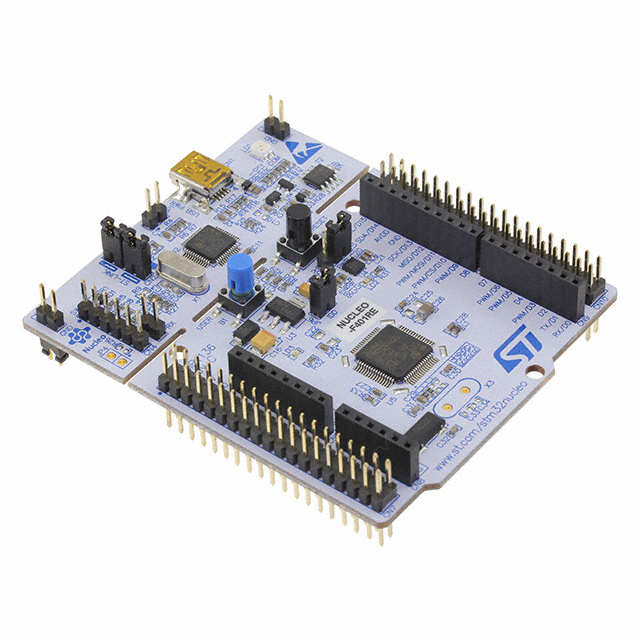
\includegraphics[scale=0.18]{images/nucleo.JPG}
    \end{figure}
\end{frame}

\subsection{Application}
\begin{frame}
    \frametitle{Application}
\begin{block}{Features}
\begin{itemize}
    \item Set temperatures over the two TEG surfaces
    \item Tune PID coefficients
    \item Visualize sensors readings and status of the micro
    \item Save all data in to log file in CSV format
\end{itemize}
\end{block}

    \begin{figure}
        \centering
        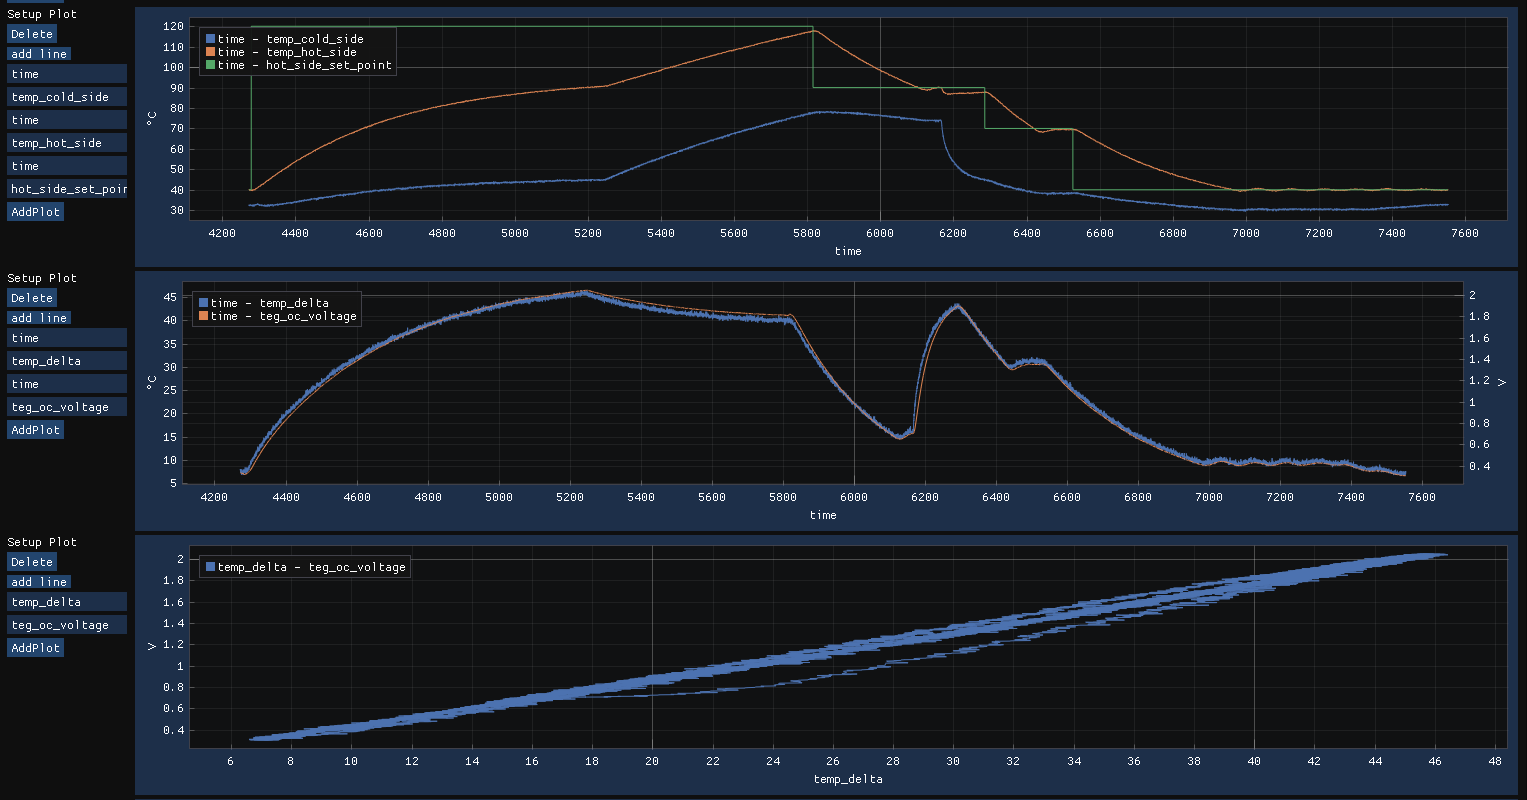
\includegraphics[scale=0.15]{images/app_plots.png}
        \caption{Plots from the GUI application}
    \end{figure}
\end{frame}

\section{Data analysis}
\subsection{Data fitting}
\begin{frame}
    \frametitle{Data fitting}

\begin{columns}[c] % The "c" option specifies centered vertical alignment while the "t" option is used for top vertical alignment
    \column{.5\textwidth}
    \begin{block}{Fit internal resistance}
        \begin{equation}
            S = \frac{V_{oc}}{\Delta T }
        \end{equation}
    \end{block}
    \begin{block}{Fit internal resistance}
        \begin{align}
            \begin{split}
            R_{int} &= R_{int_0} + R_{int_1} \cdot \overline{T} \\
            V_{OC} &= S \cdot \Delta T \\
            I &= \frac{V_{OC}}{R_{int} + R_{load}}
            \end{split}
        \end{align}
    \end{block}
\column{.5\textwidth}
\begin{figure}
    \centering
    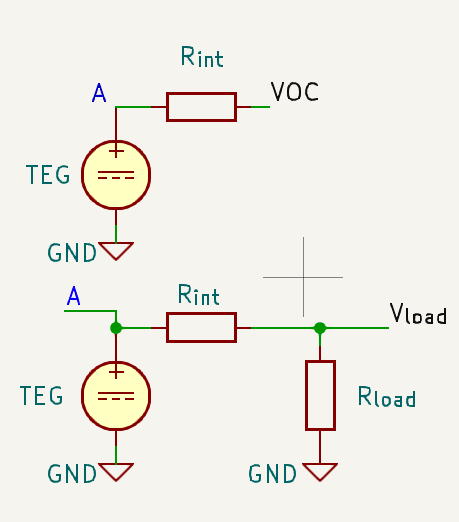
\includegraphics[width=0.9\textwidth]{images/TEGcircuitmodel.png}
    \label{fig:enter-label}
\end{figure}
\end{columns}
\begin{block}{Matlab function}
In Matlab the function fmincon allows one to fit a non-linear model with constraints on the parameters. This was used to constrain internal resistance parameters.
\end{block}
\end{frame}

\subsection{Experimental results}
\begin{frame}
    \frametitle{Experimental results}
\begin{block}{Fitted data}
    \vspace{2mm}
    \begin{tabular}{ |p{2cm}|p{2.2cm}|p{2.8cm}|  }
    \hline
    TEG model & Seebeck & Internal resistance \\ [0.5ex] 
    \hline
    \hline
    \textbf{TEG MAT} & 0.034209 & 0.145028, 0.001342\\
    \hline
    TEG 12706 & 0.044441 & 2.299155, 0.083479\\
    \hline
    TEG VL25  & 0.007100 & 0.511499, 0.004171\\
    \hline
\end{tabular}

\begin{figure}
    \centering
    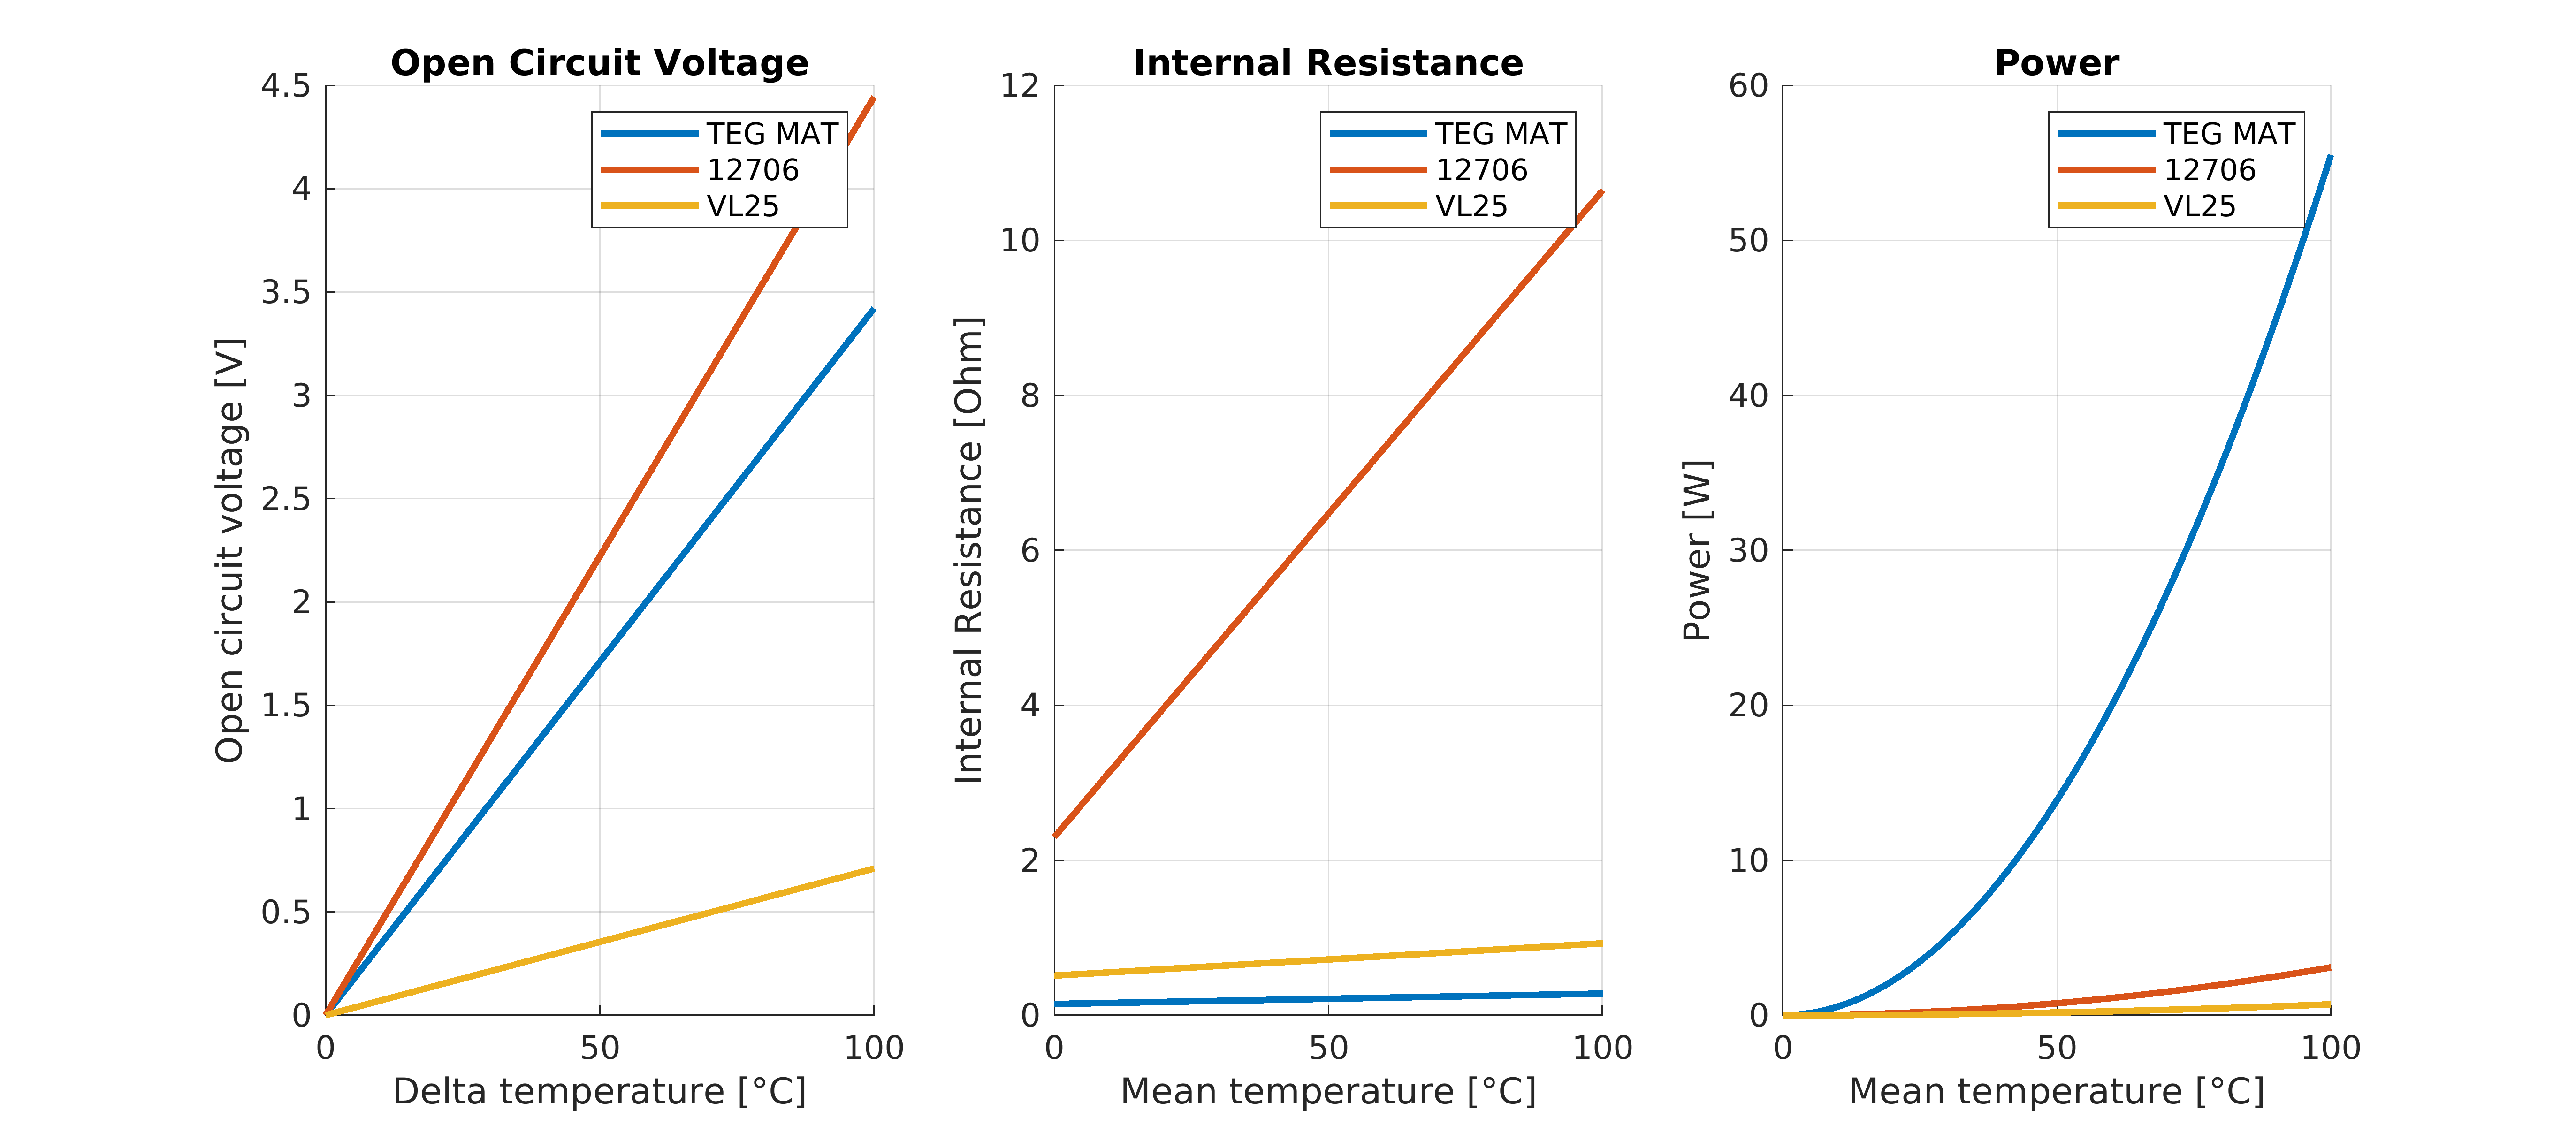
\includegraphics[width=1.0\textwidth]{images/TEGcomparison.png}
\end{figure}
\end{block}
\end{frame}

\section{Conclusion and future work}
\begin{frame}
    \frametitle{Conclusion and future work}
\begin{itemize}
    \item \textbf{Fully automated system}: the MCU must be able to automatically follow a cycle of temperatures.
    \item \textbf{Higher delta temperatures}: physical limitations prevented us from reaching high temperature deltas, either because the resistor value was too high or because the cooling system was unable to keep the cold side temperature down. 
    \item \textbf{Active cooling}: more powerful cooling system and therefore with possibility of control. 
\end{itemize}
\end{frame}

% \input{slides/02_overview}
% \input{slides/03_energy_harvesting}
% \input{slides/04_actuation_and_mechanical}
% \input{slides/05_electronics}
% \input{slides/06_software}
% \input{slides/07_autonomous_system}
% \input{slides/08_wireless_networking}
% \input{slides/09_result}
% \input{slides/10_future_works}





%\begin{frame}
%\frametitle{Overview} % Table of contents slide, comment this block out to remove it
%\tableofcontents % Throughout your presentation, if you choose to use \section{} and \subsection{} commands, these will automatically be printed on this slide as an overview of your presentation
%\end{frame}




% \begin{frame}
% \Huge{\centerline{The End}}
% \end{frame}

%----------------------------------------------------------------------------------------


\end{document} 